\scanpage{41}
\mspage{\handwritten{9}}
% archive sheet number: 40
finite with group of operators $G_j$ (resp. $G'_j$). Put, for $i\handwritten{\in}I$, $i\handwritten{>}j$, $G_i=G_j\handwritten{\times}_{S_j}S_i$ and $G=G_j\handwritten{\times}_{S_j}S$, and define similarly $G'_i$, $G'$, $H_i$,$H$, $H'_i$, and $H'$. Denote by $\operatorname{Dihom}_{S\text{-gr.}}((G,\handwritten{\unsure{H|H'|\mathbb{H}|\mathbb{H}'}}),(\handwritten{G}',H'))$ the set of di-morphisms of $S$-groups and of $S$-preschemes with group of operators from the pair $(G,H)$ to the pair $(G',H')$. Then the canonical map from $\underset{i\handwritten{\geqslant}j}{\underset{\handwritten{\longrightarrow}}{\lim}}{\unsure{B|D|\mathbb{D}}\mathrm{ihom}}_{S_i\text{-gr.}}((G_i,H_i),(G'_i,H'_i))$ to $\operatorname{Dihom}_{S\text{-gr.}}((G,H),(G',H'))$ is bijective.

(ii) In the situation recalled at the beginning of (10.0), let $G$ be an $S$-group \deleted{\unsure{finite}} of finite presentation and $H$ an $S$-prescheme of finite presentation with group of operators $G$; there then exist an index $j\handwritten{\in}J$, an $S_j$-group of finite presentation $G_j$, an $S_j$-prescheme of finite presentation $H_j$ with group of operators $G_j$ and a di-isomorphism of $S$-groups and of $S$-preschemes with groups of operators from $(G_j\handwritten{\times}_{S_j}S,H_j\handwritten{\times}_{S_j}S)$ onto$(G,H)$

\deleted{Proposition}\inserted{Definition} 10.15.- Given an $S$-functor in groups $G$ and an $S$-functor $H$ with group of operato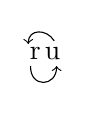
\begin{tikzpicture}[baseline=(r.base)]
\node[anchor=base,inner sep=0pt] (r) at (0,0) {r};
\node[anchor=base,inner sep=0pt] at (.22,0) {u};
\handwritten{\draw[->] (.24,.24) .. controls (.14,.40) and (-.09,.39) .. (-.09,.20);
\draw[->] (-.06,-.08) .. controls (-.07,-.36) and (.27,-.35) .. (.27,-.08);}
\end{tikzpicture}s $G$, one says that $H$ is an \uline{$S$-functor in homogeneous spaces under $G$ for the topology $\handwritten{\mathbb{T}}$}, if the canonical morphism $G\handwritten{\times}_S H\handwritten{\longrightarrow}H\handwritten{\times}_S H$ (defined by $(g,h)\handwritten{\rightsquigarrow}(g.h,h)$ for $g\handwritten{\in}G(T)$, $h\handwritten{\in}H(T)$) is an epimorphism of sheaves for the topology $\handwritten{\mathbb{T}}$.

If $G$ is an $S$-group and if $H$ is an $S$-prescheme with \deleted{group} group of operators $G$, to say that $H$ is an $S$-prescheme in homogeneous spaces under $G$ for the topology $\handwritten{\mathbb{T}}$ thus amounts to saying that the canonical morphism $G\handwritten{\times}_S H\handwritten{\longrightarrow}H\handwritten{\times}_S H$ defined as before is covering for the topology $\handwritten{\mathbb{T}}$ (\deleted{Exposé} IV 4.4.3).

Likewise, to say that an $S$-prescheme $H$ with an $S$-group $G$ as group of operators is a principal homogeneous f\deleted{o}\inserted{i}bre bundle under $G$ for the topology $\handwritten{\mathbb{T}}$ (\deleted{Exposé} IV 5.1.5) amounts to saying (\deleted{Exposé} IV 5.6 (ii)) that the canonical morphism $G\handwritten{\times}_S H\handwritten{\longrightarrow}H\handwritten{\times}_S H$ is an isomorphism and that the structure morphism $H\handwritten{\longrightarrow}S$ is covering for the topology $\handwritten{\mathbb{T}}$.

\uline{10.16.- In the situation recalled at the beginning of (10.0) , let $j\handwritten{\in}I$, $G_j$ be an $S_j$-grou-}
% The final word continues on the next scan in this package.
